% python3 code_to_tex.py gemms.py gemms_tex && xelatex </dev/null spork_gemm.tex
\documentclass[12pt]{article}

\usepackage[a5paper, landscape, margin=10mm]{geometry}
\usepackage{enumitem}
\usepackage{amsmath}
\usepackage{amssymb}
\usepackage{amsfonts}
\usepackage{placeins}
\usepackage{graphicx}
\usepackage{listings}
\usepackage{caption}
\usepackage{colortbl}
\usepackage[parfill]{parskip}
\usepackage[mathscr]{euscript}
\usepackage[usenames,dvipsnames,svgnames,table,hyperref]{xcolor}
\usepackage[hidelinks]{hyperref}
\usepackage{fontspec}
\usepackage{mdframed}

\setsansfont{FreeSans}
\setmonofont{Ubuntu Mono}
\renewcommand{\familydefault}{\sfdefault}

\hyphenation{WebGL}

\definecolor{webColor}{RGB}{0, 108, 174}
\newcommand{\web}[1]{{\color{webColor} \small \url{#1}}}
\newcommand{\webText}[2]{{\color{webColor} \href{#2}{#1}}}
\newcommand{\email}[2]{{\small \color{webColor} \textsf{\href{mailto:#1@#2}{#1[at]#2}}}}
\definecolor{titleColor}{RGB}{179, 0, 149}
\newcommand{\myTitle}[1]{{\large \color{titleColor} \hspace{-4mm} \textbf{\textsf{#1}}}}
\definecolor{subColor}{RGB}{179, 0, 149}
\newcommand{\mySub}[1]{\textsf{\color{subColor}#1}}
\definecolor{keyColor}{RGB}{170, 149, 0}
\newcommand{\myKey}[1]{\textbf{\color{keyColor}#1}}

\definecolor{redBoxFg}{RGB}{255, 0, 0}
\definecolor{redBoxBg}{RGB}{255, 218, 232}
\newcommand{\redBox}[1]{{\color{redBoxFg}\colorbox{redBoxBg}{#1}}}
\definecolor{yellowBoxFg}{RGB}{0, 0, 0}
\definecolor{yellowBoxBg}{RGB}{255, 232, 0}
\newcommand{\yellowBox}[1]{{\color{yellowBoxFg}\colorbox{yellowBoxBg}{#1}}}
\definecolor{greenBoxFg}{RGB}{0, 0, 0}
\definecolor{greenBoxBg}{RGB}{134, 210, 153}
\newcommand{\greenBox}[1]{{\color{greenBoxFg}\colorbox{greenBoxBg}{#1}}}
\definecolor{blueBoxFg}{RGB}{0, 0, 255}
\definecolor{blueBoxBg}{RGB}{218, 232, 255}
\newcommand{\blueBox}[1]{{\color{blueBoxFg}\colorbox{blueBoxBg}{#1}}}
\definecolor{violetBoxFg}{RGB}{0, 0, 0}
\definecolor{violetBoxBg}{RGB}{218, 204, 255}
\newcommand{\violetBox}[1]{{\color{violetBoxFg}\colorbox{violetBoxBg}{#1}}}

\mdfdefinestyle{MyFrame}{%
    linecolor=black,
    outerlinewidth=0pt,
    linewidth=0pt,
    innertopmargin=2.7pt,
    innerbottommargin=0pt,
    innerrightmargin=0pt,
    innerleftmargin=0pt,
        leftmargin = 0pt,
        rightmargin = 0pt}

\definecolor{lightttColor}{RGB}{69, 69, 80}
\newcommand{\lighttt}[1]{{\color{lightttColor}\texttt{#1}}}

\renewcommand*\labelenumi{(\theenumi)}
\renewcommand*{\theenumii}{\roman{enumii}}
\renewcommand*\labelenumii{\theenumii.}

\newcommand{\fixminipage}{\raggedright \setlength{\parskip}{0.3\baselineskip}}
\newcommand{\codeminipage}{\raggedright \setlength{\parskip}{0\baselineskip}}
\sloppy
\pagenumbering{gobble}


\begin{document}

\tikzstyle{smallnode} = [rectangle, minimum width=1.25cm, minimum height=1cm, text centered, text width=1.25cm, draw=black, fill=white]
\tikzstyle{smallishnode} = [rectangle, minimum width=2cm, minimum height=1cm, text centered, text width=2cm, draw=black, fill=white]
\tikzstyle{normalnode} = [rectangle, minimum width=3cm, minimum height=1cm, text centered, text width=3cm, draw=black, fill=white]
\tikzstyle{widenode} = [rectangle, minimum width=62mm, minimum height=8mm, text centered, text width=62mm, draw=black, fill=white]
\tikzstyle{bignode} = [rectangle, minimum width=3.5cm, minimum height=2cm, text centered, text width=3cm, draw=black, fill=white]
\tikzstyle{smemnode} = [rectangle, minimum width=3cm, minimum height=1cm, text centered, text width=3cm, draw=keyColorB, fill=white]
\tikzstyle{gmemnode} = [rectangle, minimum width=3cm, minimum height=1cm, text centered, text width=3cm, draw=keyColorA, fill=white]
\tikzstyle{smallishsmemnode} = [rectangle, minimum width=2cm, minimum height=1cm, text centered, text width=2cm, draw=keyColorB, fill=white]
\tikzstyle{arrow} = [thick,->,>=stealth]
\tikzstyle{line} = [thick]

\tikzstyle{rednode} = [normalnode, draw=redBoxFg, fill=redBoxBg, text=redBoxFg]
\tikzstyle{yellownode} = [normalnode, draw=yellowBoxFg, fill=yellowBoxBg, text=yellowBoxFg]
\tikzstyle{greennode} = [normalnode, draw=greenBoxFg, fill=greenBoxBg, text=greenBoxFg]
\tikzstyle{bluenode} = [normalnode, draw=blueBoxFg, fill=blueBoxBg, text=blueBoxFg]
\tikzstyle{violetnode} = [normalnode, draw=violetBoxFg, fill=violetBoxBg, text=violetBoxFg]

\tikzstyle{Mnode} = [greennode, text width=55mm, minimum width=55mm, minimum height=7mm]
\tikzstyle{Nnode} = [violetnode, text width=7mm, minimum width=7mm, minimum height=7mm]

\tikzstyle{producer} = [yellownode, text width=64mm, minimum width=64mm, minimum height=14mm]
\tikzstyle{consumer} = [greennode, text width=20mm, minimum width=20mm, minimum height=14mm]
\tikzstyle{smallproducer} = [yellownode, text width=20mm, minimum width=20mm, minimum height=14mm]
\tikzstyle{copylatency} = [rednode, text width=84mm, minimum width=84mm, minimum height=8mm]
\tikzstyle{ring} = [rednode, text width=16mm, minimum width=1mm, minimum height=14mm]
\newcommand{\consumerBox}[1]{{\color{greenBoxFg}\colorbox{greenBoxBg}{#1}}}
\newcommand{\producerBox}[1]{{\color{yellowBoxFg}\colorbox{yellowBoxBg}{#1}}}

{ \LARGE Exo Dev 2025-05-06 } \hfill { \LARGE \textbf{\textsf{Spork: GEMM Samples}}}

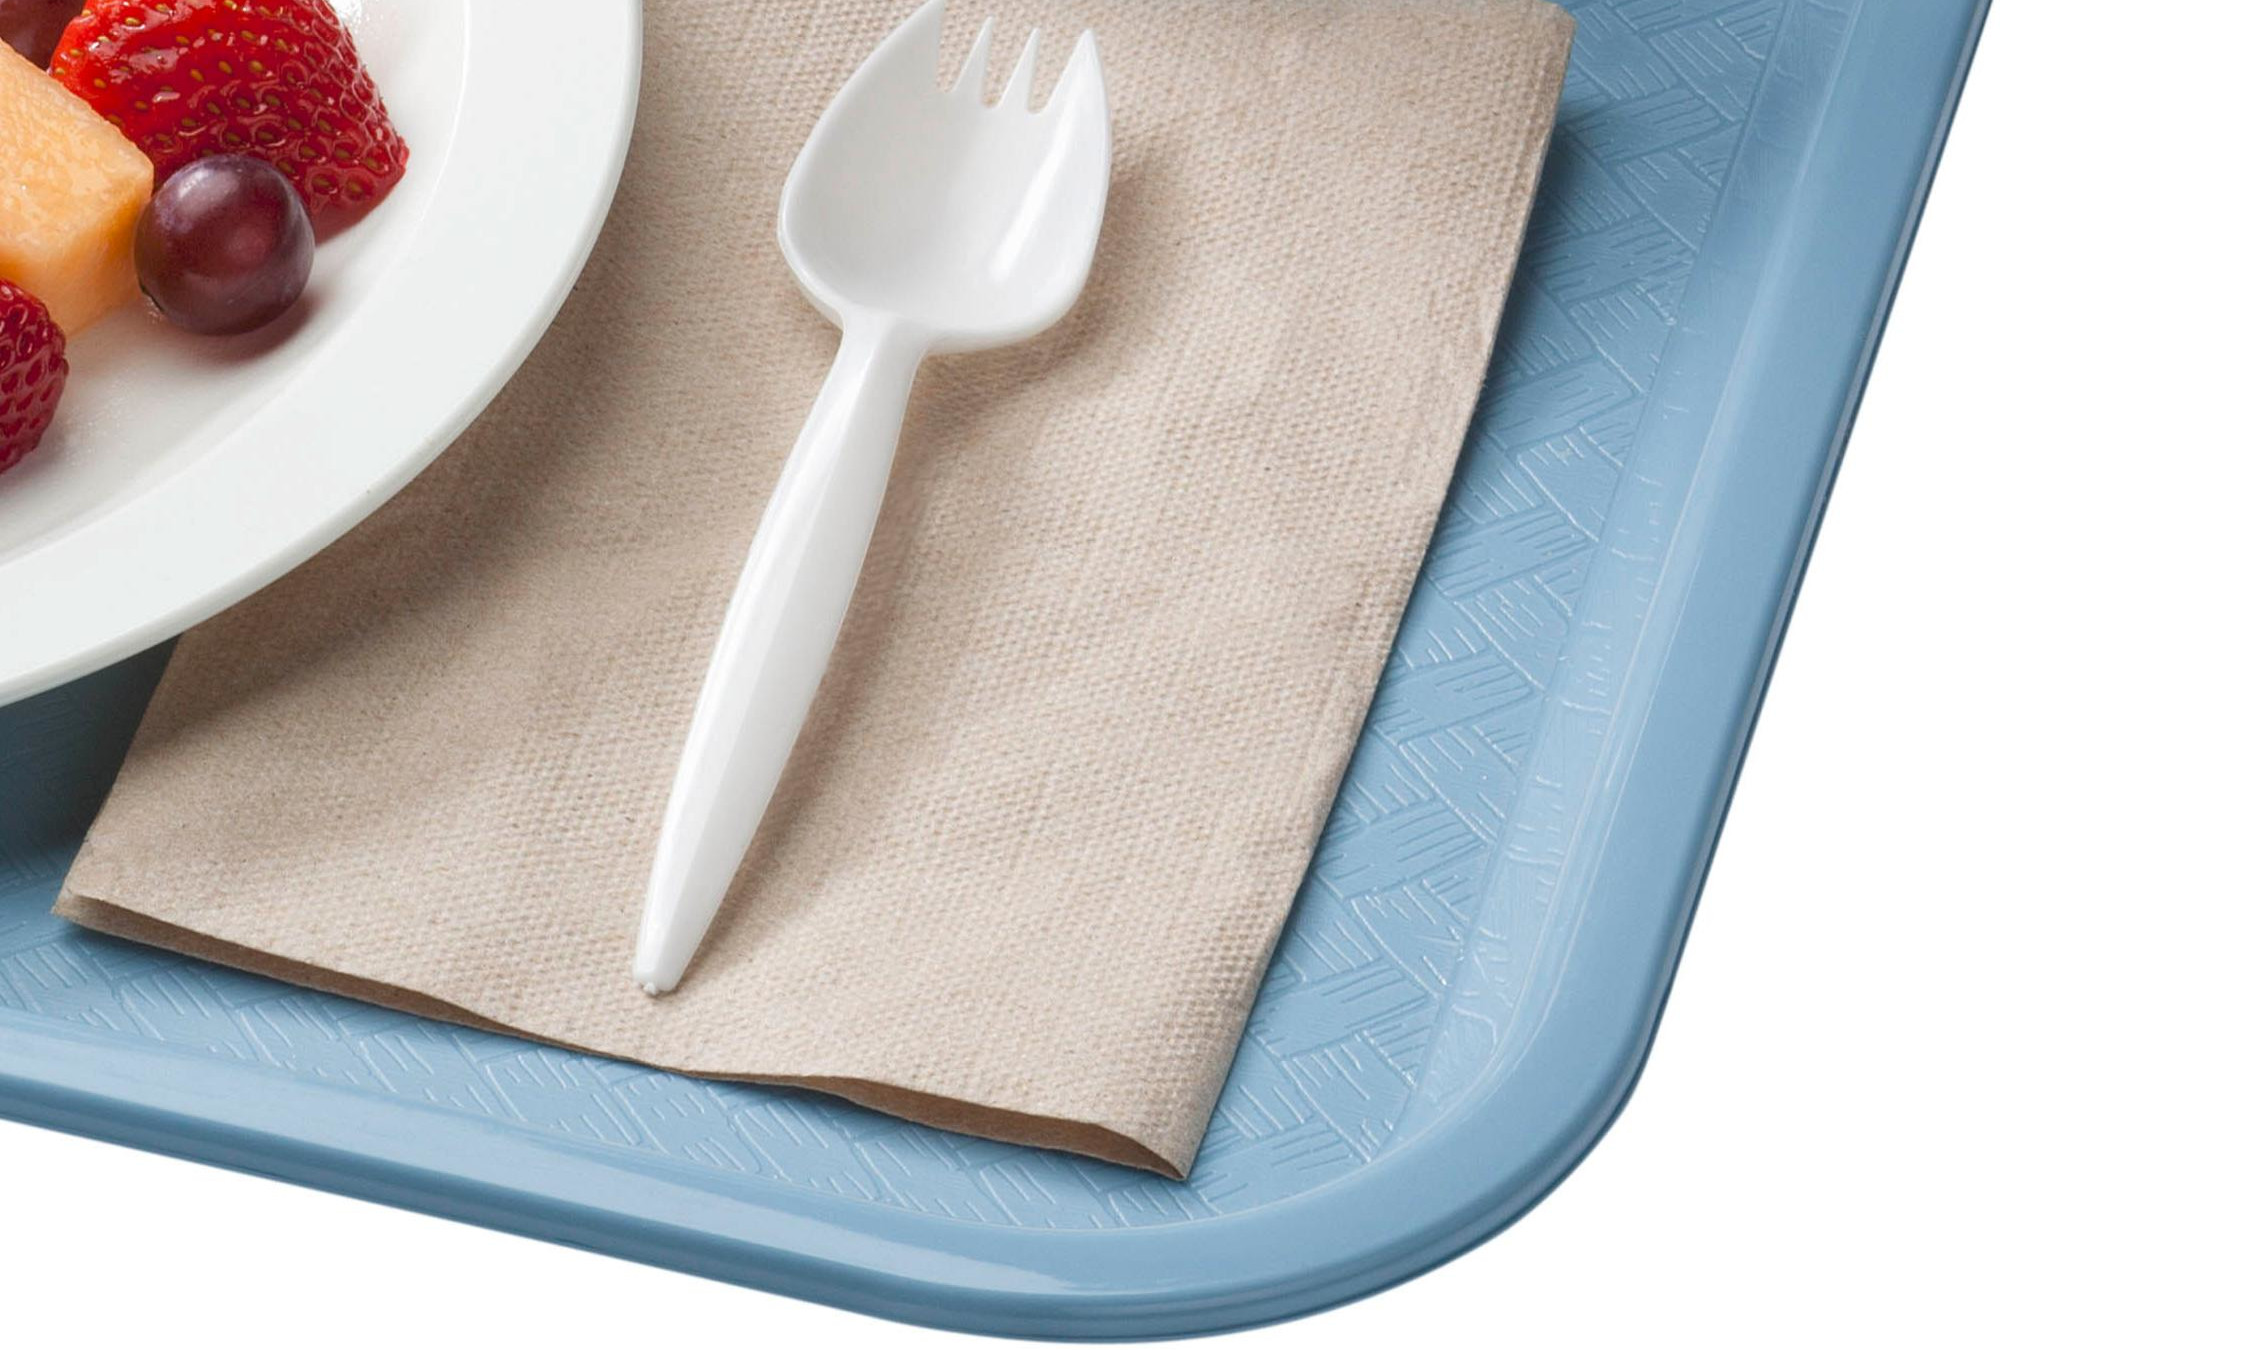
\includegraphics[width=\linewidth]{usda_spork.jpg}

\newpage
\myTitle{Basic Concepts}

\begin{minipage}[t]{0.48\textwidth}\fixminipage

Exo: Python-embedded DSL with mostly sequential semantics.
Syntax lowers $\approx 1:1$ to C.

Exo-GPU annotates Exo with parallelization directives.

%% Scheduling checks will retain sequential semantics.
%% ``Prove'' at the end that the scheduled function, as a sequential program, behaves the same as the parallelized program.

\mySub{Language Constructs for GPUs}
\begin{itemize}
  \item Parallel for loops
  \item Add sync statements
  \item Add GPU memory types (Exo annotates memory types as \texttt{var @ \redBox{memory}})
\end{itemize}

\mySub{Goals}
\begin{itemize}
  \item Imperatively program individual threads
  \item Support async instructions
  \item ...but type systems watch over our imperative programing
\end{itemize}

\mySub{Not in this talk}
\begin{itemize}
  \item Scheduling semantics (still sequential)
  \item Sequential-parallel equivalence
  \item (i.e. ``prove'' that parallel program + syncs = sequential program behavior)
\end{itemize}
\end{minipage}
\hfill
\begin{minipage}[t]{0.48\textwidth}\fixminipage

Each statement of an Exo-GPU program has these 2 static properties:

\mySub{Actor Kind}

Intuitively, the ``timeline'' the statement runs on
\begin{itemize}
  \item \texttt{cpu}: host CPU
  \item \texttt{cuda\_classic}: most CUDA device code
  \item async CUDA instructions
\end{itemize}
\texttt{with CudaDeviceFunction} wraps CUDA code.\\
Changes the actor kind from \texttt{cpu} to \texttt{cuda\_classic}

\mySub{Collective Unit}

Number and arrangement of threads cooperating to execute a statement

e.g. thread, warp, CTA, or user-defined \# threads

Manipulated with parallel for loops

\begin{itemize}
  \item \texttt{cuda\_tasks}: outer loops, allocate work to CTAs (or clusters)
  \item \texttt{cuda\_threads}: inner loops, allocate sub-CTA work to threads
\end{itemize}
\end{minipage}

\newpage
\myTitle{Starter Example: Actor Kinds}

Output stationary example: each thread computes one value of the output matrix $C$.

Threads grouped into 256 thread CTAs that compute a $16 \times 16$ tile.

\input{gemms_tex/intro.0.tex}
\newpage
\myTitle{Starter Example: Memory Types}

\input{gemms_tex/intro.1.tex}

\newpage
\myTitle{Starter Example: Collective Units}

\input{gemms_tex/intro.2.tex}

\newpage
\myTitle{cuda\_threads Loop Example}

\input{gemms_tex/par.0.tex}

\begin{tikzpicture}[node distance=2mm]
\node (cta) [yellownode, minimum width=30mm, minimum height=40mm] {CTA: 256 threads};

\node (m2) [Mnode, right=of cta, xshift=16mm] {\texttt{m1 = 2}; threads [32, 47]};
\node (m1) [Mnode, above=of m2] {\texttt{m1 = 1}; threads [16, 31]};
\node (m0) [Mnode, above=of m1] {\texttt{m1 = 0}; threads [0, 15]};
\node (m15) [Mnode, below=of m2, yshift=-9mm] {\texttt{m1 = 15}; threads [240, 255]};
\draw [arrow] (cta) -- node[above] {\texttt{for \redBox{m1}}} (m2);
\draw [dotted] (m2) -- (m15);
\node (m0n0) [Nnode, right=of m0, xshift=16mm] {0};
\node (m0n1) [Nnode, right=of m0n0] {1};
\node (m0n2) [Nnode, right=of m0n1] {2};
\node (m0n15) [Nnode, right=of m0n2, xshift=8mm] {15};
\node (m1n0) [Nnode, below=of m0n0] {16};
\node (m1n1) [Nnode, below=of m0n1] {17};
\node (m1n2) [Nnode, below=of m0n2] {18};
\node (m1n15) [Nnode, below=of m0n15] {31};
\node (m2n0) [Nnode, below=of m1n0] {32};
\node (m2n1) [Nnode, below=of m1n1] {33};
\node (m2n2) [Nnode, below=of m1n2] {34};
\node (m2n15) [Nnode, below=of m1n15] {47};
\node (m15n0) [Nnode, right=of m15, xshift=16mm] {240};
\node (m15n1) [Nnode, right=of m15n0] {241};
\node (m15n2) [Nnode, right=of m15n1] {242};
\node (m15n15) [Nnode, right=of m15n2, xshift=8mm] {255};
\draw [arrow] (m0) -- node[above] {\texttt{for \blueBox{n1}}} (m0n0);
\draw [arrow] (m1) -- node[above] {\texttt{for \blueBox{n1}}} (m1n0);
\draw [arrow] (m2) -- node[above] {\texttt{for \blueBox{n1}}} (m2n0);
\draw [arrow] (m15) -- node[below] {\texttt{for \blueBox{n1}}} (m15n0);
\draw [dotted] (m2n0) -- node[] {\texttt{n1=0}} (m15n0);
\draw [dotted] (m2n1) -- node[] {\texttt{n1=1}} (m15n1);
\draw [dotted] (m2n2) -- node[] {\texttt{n1=2}} (m15n2);
\draw [dotted] (m2n15) --node[] {\texttt{n1=15}} (m15n15);
\draw [dotted] (m0n2) -- (m0n15);
\draw [dotted] (m1n2) -- (m1n15);
\draw [dotted] (m2n2) -- (m2n15);
\draw [dotted] (m15n2) -- (m15n15);

\end{tikzpicture}

\newpage
\myTitle{Register Tiles: Assign Multiple Output Values to 1 Thread}

\input{gemms_tex/tile.0.tex}
\newpage
\myTitle{Tile 1}

\input{gemms_tex/tile.1.tex}

\newpage
\myTitle{Tile 2}

\input{gemms_tex/tile.2.tex}

\newpage
\myTitle{SMEM Tile Reuse}

All threads are reading directly from GMEM (global memory), which misses important re-use opportunities.

\input{gemms_tex/gmem_remark.0.tex}

\newpage
\myTitle{SMEM Tile Reuse}

Decompose the CTA's output $C$ matrix tile as a sum of $A$, $B$ matrix tile products

The CTA's threads alternate between
\begin{itemize}
  \item Cooperatively loading $A$, $B$ tiles to \myKeyB{SMEM} (shared memory; per-CTA scratchpad): ``produce''
  \item Cooperatively accumulating loaded SMEM tiles: ``consume''
\end{itemize}
We need to insert syncs to make the cooperation work.

% This is so janky...
\begin{tikzpicture}[node distance=2mm]
\node (c) [normalnode, minimum width=50mm, minimum height=50mm] { $C$ };
\node (eq) [right=of c] {$=$};
\node (a) [normalnode, minimum width=50mm, minimum height=50mm, right=of eq] { $A$ };
\node (b) [normalnode, minimum width=50mm, minimum height=50mm, right=of a] { $B$ };
\node (c0) [rednode, minimum width=10mm, minimum height=10mm, text width=10mm, xshift=-10mm, yshift=10mm] {\texttt{accum}};
\node (a0) [greennode, minimum width=5mm, minimum height=10mm, text width=0mm, right=of c0, xshift=38mm] {};
\node (a1) [greennode, minimum width=5mm, minimum height=10mm, text width=0mm, right=of a0] {};
\node (a2) [greennode, minimum width=5mm, minimum height=10mm, text width=0mm, right=of a1] {};
\node (a3) [greennode, minimum width=5mm, minimum height=10mm, text width=0mm, right=of a2] {};
\node (a4) [greennode, minimum width=5mm, minimum height=10mm, text width=0mm, right=of a3] {};
\node (a5) [greennode, minimum width=5mm, minimum height=10mm, text width=0mm, right=of a4] {};
\node (a6) [greennode, minimum width=5mm, minimum height=10mm, text width=0mm, right=of a5] {};
\node (b0) [violetnode, minimum width=10mm, minimum height=5mm, text width=10mm, right=of a6, xshift=9mm, yshift=11.5mm] {};
\node (b1) [violetnode, minimum width=10mm, minimum height=5mm, text width=10mm, below=of b0] {};
\node (b2) [violetnode, minimum width=10mm, minimum height=5mm, text width=10mm, below=of b1] {};
\node (b3) [violetnode, minimum width=10mm, minimum height=5mm, text width=10mm, below=of b2] {};
\node (b4) [violetnode, minimum width=10mm, minimum height=5mm, text width=10mm, below=of b3] {};
\node (b5) [violetnode, minimum width=10mm, minimum height=5mm, text width=10mm, below=of b4] {};
\node (b6) [violetnode, minimum width=10mm, minimum height=5mm, text width=10mm, below=of b5] {};
\end{tikzpicture}

\newpage
\myTitle{SMEM Tile Reuse}

Divide $k$ accumulation loop by K-block size (32 in these examples)

Outer \blueBox{\texttt{k1}} loop over matrix blocks; inner \blueBox{\texttt{k0}} loop handles block-block multiplication.

\begin{minipage}[t]{0.48\textwidth}\fixminipage
\begin{itemize}
  \item Zero-initialize accumulator
  \item \texttt{k1 = 0}: threads cooperate to load A, B tiles (offset $k = 0$)
  \item Sync threads
  \item \texttt{k1 = 0}: threads multiply-accum A, B tiles
  \item Sync threads
  \item \texttt{k1 = 1}: threads cooperate to load A, B tiles (offset $k = 32$)
  \item Sync threads
  \item \texttt{k1 = 1}: threads multiply-accum A, B tiles
  \item Sync threads
  \item \texttt{k1 = 2}: threads cooperate to load A, B tiles (offset $k = 64$)
  \item Sync threads
  \item \texttt{k1 = 2}: threads multiply-accum A, B tiles
  \item ...
\end{itemize}
\end{minipage}
\hfill
\begin{minipage}[t]{0.48\textwidth}\fixminipage
~\\
\begin{tikzpicture}[node distance=0mm]
\node (c0) [normalnode, minimum width=25mm, minimum height=25mm, text width=6mm] { $C$ };
\node (accum0) [rednode, minimum width=5mm, minimum height=5mm, text width=0mm, left=of c0, xshift=10mm, yshift=5mm] {};
\node (p0) [right=of c0] {\texttt{+=}};
\node (a0) [normalnode, minimum width=25mm, minimum height=25mm, text width=6mm, right=of p0] { $A$ };
\node (aT0) [greennode, minimum width=5mm, minimum height=5mm, text width=0mm, left=of a0, xshift=5mm, yshift=5mm] {};
\node (b0) [normalnode, minimum width=25mm, minimum height=25mm, text width=6mm, right=of a0, xshift=2mm] { $B$ };
\node (bT0) [violetnode, minimum width=5mm, minimum height=5mm, text width=0mm, left=of b0, xshift=10mm, yshift=10mm] {};

\node (c1) [normalnode, minimum width=25mm, minimum height=25mm, text width=6mm, below=of c0, yshift=-4mm] { $C$ };
\node (accum1) [rednode, minimum width=5mm, minimum height=5mm, text width=0mm, left=of c1, xshift=10mm, yshift=5mm] {};
\node (p1) [right=of c1] {\texttt{+=}};
\node (a1) [normalnode, minimum width=25mm, minimum height=25mm, text width=6mm, right=of p1] { $A$ };
\node (aT1) [greennode, minimum width=5mm, minimum height=5mm, text width=0mm, left=of a1, xshift=10mm, yshift=5mm] {};
\node (b1) [normalnode, minimum width=25mm, minimum height=25mm, text width=6mm, right=of a1, xshift=2mm] { $B$ };
\node (bT1) [violetnode, minimum width=5mm, minimum height=5mm, text width=0mm, left=of b1, xshift=10mm, yshift=5mm] {};

\node (c2) [normalnode, minimum width=25mm, minimum height=25mm, text width=6mm, below=of c1, yshift=-4mm] { $C$ };
\node (accum2) [rednode, minimum width=5mm, minimum height=5mm, text width=0mm, left=of c2, xshift=10mm, yshift=5mm] {};
\node (p2) [right=of c2] {\texttt{+=}};
\node (a2) [normalnode, minimum width=25mm, minimum height=25mm, text width=6mm, right=of p2] { $A$ };
\node (aT2) [greennode, minimum width=5mm, minimum height=5mm, text width=0mm, left=of a2, xshift=15mm, yshift=5mm] {};
\node (b2) [normalnode, minimum width=25mm, minimum height=25mm, text width=6mm, right=of a2, xshift=2mm] { $B$ };
\node (bT2) [violetnode, minimum width=5mm, minimum height=5mm, text width=0mm, left=of b2, xshift=10mm, yshift=0mm] {};

\end{tikzpicture}
\end{minipage}

\newpage
\myTitle{SMEM Tile Sizing}

When we choose the tile sizes for $A$ and $B$, generally, $M, N > K$.\\
This maximizes re-use when multiplying the two tiles.

\begin{tikzpicture}[node distance=0mm]
\node (cL) [normalnode, minimum width=50mm, minimum height=50mm] {};
\node (aL) [smallnode, minimum width=20mm, minimum height=50mm, left=of cL, xshift=-2mm] {$A$};
\node (aRow) [greennode, minimum width=18mm, minimum height=6mm, above=of aL, yshift=-18mm, text width=0mm] {};
\node (bL) [smallnode, minimum width=50mm, minimum height=20mm, above=of cL, yshift=2mm] {$B$};
\draw (aRow.east) to[out=0, in=270] ($(bL.south) - (2.0, 0)$);
\draw (aRow.east) to[out=0, in=270] ($(bL.south) - (1.2, 0)$);
\draw (aRow.east) to[out=0, in=270] ($(bL.south) - (0.4, 0)$);
\draw (aRow.east) to[out=0, in=270] ($(bL.south) + (0.4, 0)$);
\draw (aRow.east) to[out=0, in=270] ($(bL.south) + (1.2, 0)$);
\draw (aRow.east) to[out=0, in=270] ($(bL.south) + (2.0, 0)$);
\node (ML) [right=of aL, xshift=2mm] {\greenBox{$M$}};
\node (NL) [below=of bL, yshift=-2mm] {\violetBox{$N$}};
\node (aKL) [above=of aL] {\blueBox{$K$}};
\node (bKL) [left=of bL] {\blueBox{$K$}};
\node (Lcaption) [below=of cL, xshift=-11mm] {Each row of the $A$ tile is used \violetBox{$N$} times.};

\node (cR) [normalnode, minimum width=50mm, minimum height=50mm, right=of cL, xshift=42mm] {};
\node (aR) [smallnode, minimum width=20mm, minimum height=50mm, left=of cR, xshift=-2mm] {$A$};
\node (bR) [smallnode, minimum width=50mm, minimum height=20mm, above=of cR, yshift=2mm] {$B$};
\node (bCol) [violetnode, minimum width=6mm, minimum height=18mm, left=of bR, xshift=18mm, text width=0mm] {};
\draw (bCol.south) to[out=270, in=0] ($(aR.east) - (0, 2.0)$);
\draw (bCol.south) to[out=270, in=0] ($(aR.east) - (0, 1.2)$);
\draw (bCol.south) to[out=270, in=0] ($(aR.east) - (0, 0.4)$);
\draw (bCol.south) to[out=270, in=0] ($(aR.east) + (0, 0.4)$);
\draw (bCol.south) to[out=270, in=0] ($(aR.east) + (0, 1.2)$);
\draw (bCol.south) to[out=270, in=0] ($(aR.east) + (0, 2.0)$);
\node (MR) [right=of aR, xshift=2mm] {\greenBox{$M$}};
\node (NR) [below=of bR, yshift=-2mm] {\violetBox{$N$}};
\node (aKR) [above=of aR] {\blueBox{$K$}};
\node (bKR) [left=of bR] {\blueBox{$K$}};
\node (Rcaption) [below=of cR, xshift=-11mm] {Each column of the $B$ tile is used \greenBox{$M$} times.};
\end{tikzpicture}


In contrast, increasing the \blueBox{$K$} tile size yields no re-use.


\newpage
\myTitle{SMEM Alloc}

\input{gemms_tex/smem_alloc.0.tex}

\texttt{Fence(cuda\_classic, cuda\_classic)} is an all-threads-to-all-threads sync in Exo-GPU, where ``all'' is defined by the collective unit.

\texttt{cuda\_classic}: actor kind; for now, we don't need to worry about this.

\newpage
\myTitle{Broken SMEM 0}

\input{gemms_tex/broken_smem.0.tex}

\newpage
\myTitle{Broken SMEM 1}

\input{gemms_tex/broken_smem.1.tex}

\newpage
\myTitle{Broken SMEM 2}

\input{gemms_tex/broken_smem.2.tex}

\newpage
\myTitle{Distributed Memory 0}

\input{gemms_tex/dmem.0.tex}

\newpage
\myTitle{Distributed Memory 1}

\input{gemms_tex/dmem.1.tex}

\newpage
\myTitle{Distributed Memory 2}

\input{gemms_tex/dmem.2.tex}

\newpage
\myTitle{Distributed Memory 3}

\input{gemms_tex/dmem.3.tex}

\newpage
\myTitle{Distributed Memory 4}

\input{gemms_tex/dmem.4.tex}
\newpage
\myTitle{Distributed Memory 5}

\begin{minipage}[t]{0.48\textwidth}\fixminipage
\mySub{Before}

\input{gemms_tex/dmem_before.0.tex}
\end{minipage}
\hfill
\begin{minipage}[t]{0.48\textwidth}\fixminipage
\mySub{After}

\input{gemms_tex/dmem_after.0.tex}

\vspace{4mm}
Distributed dimensions (\blacktt{f32[\greenBox{16}, \violetBox{16}, ...]}) are elided in the generated C++ code.
\end{minipage}

All of this was just to lift the \texttt{accum} variable out of the loop!

\myKeyA{Rationale:} Why did we need to do this? (i.e. why not just lower \texttt{accum[8, 16]} verbatim)?

\begin{itemize}
  \item Sequential-parallel equivalence: parallel-fors are just ``pragmas'', shouldn't change tensor meaning
  \item Sequential scheduling language needs to understand ``intent'' and dataflow of the full tensor
  \item We also need this to be explicit for multicast instructions (not in this talk)
\end{itemize}

\newpage
\myTitle{Working SMEM Example 0}

\input{gemms_tex/working_smem.0.tex}

\newpage
\myTitle{Working SMEM Example 1}

\input{gemms_tex/working_smem.1.tex}
\newpage
\myTitle{Working SMEM Example 2}

\input{gemms_tex/working_smem.2.tex}

\newpage
\myTitle{Ring Buffer -- Why}

Hardware underutilized -- strictly separate memory (``produce'': load SMEM) and compute (``consume'': accumulate) workloads.

\begin{tikzpicture}[node distance=2mm]
\node (produce0) [producer] {Produce \texttt{k1 = 0}};
\node (consume0) [consumer, right=of produce0] {Consume \texttt{k1 = 0}};
\node (produce1) [producer, right=of consume0] {Produce \texttt{k1 = 1}};
\node (consume1) [consumer, right=of produce1] {Consume \texttt{k1 = 1}};
\end{tikzpicture}

Overlap produce and consume workloads

\begin{tikzpicture}[node distance=2mm]
\node (produce0) [producer] {Produce \texttt{k1 = 0}};
\node (consume0) [consumer, right=of produce0] {Consume \texttt{k1 = 0}};
\node (produce1) [producer, below=of produce0, xshift=24mm] {Produce \texttt{k1 = 1}};
\node (consume1) [consumer, right=of produce1] {Consume \texttt{k1 = 1}};
\node (produce2) [producer, below=of produce1, xshift=24mm] {Produce \texttt{k1 = 2}};
\node (consume2) [consumer, right=of produce2] {Consume \texttt{k1 = 2}};
\node (produce3) [producer, below=of produce2, xshift=24mm] {Produce \texttt{k1 = 3}};
\node (consume3) [consumer, right=of produce3] {Consume \texttt{k1 = 3}};
\node (produce4) [producer, below=of produce3, xshift=24mm] {Produce \texttt{k1 = 4}};
\node (consume4) [consumer, right=of produce4] {Consume \texttt{k1 = 4}};
\end{tikzpicture}

\newpage
\myTitle{Ring Buffer -- Why}

Latency of \producerBox{producer} (memory) workloads is very long compared to \consumerBox{consumer} workloads.

We need a deep ring buffer to hide latency.
Many copies are in flight simultaneously.

\begin{tikzpicture}[node distance=2mm]
\node (produce0) [producer] {Produce \texttt{k1 = 0}};
\node (consume0) [consumer, right=of produce0] {Consume \texttt{k1 = 0}};
\node (produce1) [producer, below=of produce0, xshift=24mm] {Produce \texttt{k1 = 1}};
\node (consume1) [consumer, right=of produce1] {Consume \texttt{k1 = 1}};
\node (produce2) [producer, below=of produce1, xshift=24mm] {Produce \texttt{k1 = 2}};
\node (consume2) [consumer, right=of produce2] {Consume \texttt{k1 = 2}};
\node (produce3) [producer, below=of produce2, xshift=24mm] {Produce \texttt{k1 = 3}};
\node (consume3) [consumer, right=of produce3] {Consume \texttt{k1 = 3}};
\node (produce4) [producer, right=of consume0] {Produce \texttt{k1 = 4}};
\node (consume4) [consumer, right=of produce4] {Consume \texttt{k1 = 4}};
\node (produce5) [producer, right=of consume1] {Produce \texttt{k1 = 5}};
\node (consume5) [consumer, right=of produce5] {Consume \texttt{k1 = 5}};
\node (produce6) [producer, right=of consume2] {Produce \texttt{k1 = 6}};
\node (produce7) [producer, right=of consume3] {Produce \texttt{k1 = 7}};
\node (ring0) [ring, left=of produce0] {Buffer 0};
\node (ring1) [ring, below=of ring0] {Buffer 1};
\node (ring2) [ring, below=of ring1] {Buffer 2};
\node (ring3) [ring, below=of ring2] {Buffer 3};
\draw [arrow] (produce0) to[out=45, in=135] node [above] (forward) {\violetBox{Arrive/Await}} (consume0);
\draw [arrow] (consume0) to[out=45, in=135] node [above] (forward) {\violetBox{ReverseArrive/ReverseAwait}} (produce4);
\end{tikzpicture}

Forward synchronization: Consumer \consumerBox{\texttt{k1 = N}} waits for producer \producerBox{\texttt{k1 = N}}\\
(RAW hazard: we need to wait for the SMEM tiles to be filled)

Reverse synchronization: Producer \producerBox{\texttt{k1 = N}} waits for consumer \consumerBox{\texttt{k1 = N - 4}}\\
(WAR hazard: we need to not overwrite SMEM tiles before they're fully consumed)

\newpage
\myTitle{Warp Specialization}

Dedicate some warps (32-thread groups) to be \producerBox{producers} and some to be \consumerBox{consumers}.\\
We use \blueBox{\texttt{with CudaWarps}} in Exo to control work assignment to threads.

\begin{tikzpicture}[node distance=2mm]
\node (produce0) [smallproducer] {Copy instr \texttt{k1 = 0}};
\node (produce1) [smallproducer, right=of produce0] {Copy instr \texttt{k1 = 1}};
\node (produce2) [smallproducer, right=of produce1] {Copy instr \texttt{k1 = 2}};
\node (produce3) [smallproducer, right=of produce2] {Copy instr \texttt{k1 = 3}};
\node (produce4) [smallproducer, right=of produce3] {Copy instr \texttt{k1 = 4}};
\node (produce5) [smallproducer, right=of produce4] {Copy instr \texttt{k1 = 5}};
\node (produce6) [smallproducer, right=of produce5] {Copy instr \texttt{k1 = 6}};
\node (produce7) [smallproducer, right=of produce6] {Copy instr \texttt{k1 = 7}};
\node (producers) [text width=19mm, left=of produce0] {Threads [256, 383]};
\node (copy0) [copylatency, below=of produce0, xshift=32mm] {Copy latency (to buffer 0)};
\node (copy1) [copylatency, below=of copy0, xshift=25mm] {Copy latency (to buffer 1)};
\node (copy2) [copylatency, below=of copy1, xshift=25mm] {Copy latency (to buffer 2)};
\node (copy3) [copylatency, below=of copy2, xshift=25mm] {Copy latency (to buffer 3)};
\node (copy4) [copylatency, right=of copy0, xshift=11mm] {Copy latency (to buffer 0)};
\node (copy5) [copylatency, below=of copy4, xshift=25mm] {Copy latency (to buffer 1)};
\node (copy6) [copylatency, below=of copy5, xshift=25mm] {Copy latency (to buffer 2)};
\node (copy7) [copylatency, below=of copy6, xshift=25mm] {Copy latency (to buffer 3)};
\node (consume0) [consumer, below=of copy3, xshift=-18mm] {Consume \texttt{k1 = 0}};
\node (consume1) [consumer, right=of consume0] {Consume \texttt{k1 = 1}};
\node (consume2) [consumer, right=of consume1] {Consume \texttt{k1 = 2}};
\node (consume3) [consumer, right=of consume2] {Consume \texttt{k1 = 3}};
\node (consume4) [consumer, right=of consume3] {Consume \texttt{k1 = 4}};
\node (consumer) [text width=19mm, left=of consume0] {Threads [0, 255]};

%% \draw[arrow, dotted] (produce0.south) to[out=270, in=135] (copy0.west);
%% \draw[arrow, dotted] (produce1.south) to[out=270, in=135] (copy1.west);
%% \draw[arrow, dotted] (produce2.south) to[out=270, in=135] (copy2.west);
%% \draw[arrow, dotted] (produce3.south) to[out=270, in=135] (copy3.west);
%% \draw[arrow, dotted] (produce4.south) to[out=270, in=135] (copy4.west);
%% \draw[arrow, dotted] (produce5.south) to[out=270, in=135] (copy5.west);
%% \draw[arrow, dotted] (produce6.south) to[out=270, in=135] (copy6.west);
%% \draw[arrow, dotted] (produce7.south) to[out=270, in=135] (copy7.west);

\draw[arrow, dotted] (copy0.east) to[out=315, in=90] (consume0.north);
\draw[arrow, dotted] (copy1.east) to[out=315, in=90] (consume1.north);
\draw[arrow, dotted] (copy2.east) to[out=315, in=90] (consume2.north);
\draw[arrow, dotted] (copy3.east) to[out=315, in=90] (consume3.north);
\end{tikzpicture}
%In Exo, use \texttt{with CudaWarps} to specialize threads: alters lowering of child \texttt{cuda\_threads} loops.

\begin{minipage}[t]{0.4\textwidth}\fixminipage
\input{gemms_tex/CudaWarps.0.tex}
\end{minipage}
\hfill
\begin{minipage}[t]{0.58\textwidth}\fixminipage
\input{gemms_tex/CudaWarps.1.tex}
\end{minipage}
\newpage
\myTitle{Ring Buffer Example: Thread Specialization}

\input{gemms_tex/ring.0.tex}

\newpage
\myTitle{Ring Buffer Example: Producer Threads Detail}

\input{gemms_tex/ring.1.tex}

\newpage
\myTitle{Ring Buffer Example: Consumer Threads Detail}

\input{gemms_tex/ring.2.tex}

\newpage
\myTitle{Problem With Copies}

\input{gemms_tex/sync_copy.0.tex}

\newpage
\myTitle{TMA (Bulk Copy) Instructions}

\begin{minipage}[t]{0.48\textwidth}\fixminipage
\begin{itemize}
\item A single \texttt{cp.bulk.async} instruction can copy a large 1D-5D tile \myKey{GMEM}$\leftrightarrow$\myKeyB{SMEM}
\item \myKeyB{SMEM} tile: densely packed C-order matrix
\begin{itemize}
  \item 128 byte alignment
\end{itemize}
\item \myKey{GMEM} tile: tile from big C-order matrix
\begin{itemize}
  \item \myKey{Predicated} and strided
  \item 16 byte aligned memory and strides
\end{itemize}
\end{itemize}

\begin{tikzpicture}[node distance=5mm]
\node (smem) [smemnode] {\myKeyB{SMEM tile}};
\node (gmembig) [bignode, right=of smem, yshift=-3mm] {};
\node (gmem) [gmemnode, right=of smem, xshift=9mm] {\myKey{GMEM tile}};
\draw [arrow] ($(smem.east)-(0,0.2)$) -- ($(gmem.west)-(0,0.2)$);
\draw [arrow] ($(gmem.west)+(0,0.2)$) -- ($(smem.east)+(0,0.2)$);
\end{tikzpicture}
\end{minipage}
\hfill
\begin{minipage}[t]{0.48\textwidth}\fixminipage
\mySub{Contrast with synchronous copy instructions}
\begin{itemize}
  \item Copies large tiles instead of only 4/8/16 bytes at a time.
  \item Bypasses registers
  \item Async copy: execution continues \textit{without waiting for copy to finish}
  \item Async copies don't interact with normal synchronization, e.g. \texttt{\_\_syncthreads();}
\end{itemize}

\mySub{Actor Kind}

Exo-GPU will categorize instructions based on \myKeyA{actor kind}; essentially, instructions that operate on different timelines have different actor kinds.
\begin{itemize}
  \item \texttt{cpu}: CPU instructions
  \item \texttt{cuda\_classic}: CUDA non-async instr
  \item \texttt{tma\_to\_smem\_async}: async copies to SMEM
  \item \texttt{wgmma\_async}: Async H100 tensor core
  \item ...
\end{itemize}
Parameterize sync statements (Fence/Arrive/Await) with \myKeyA{actor kind}; lowers to barriers that target a specific instruction category.
\end{minipage}

\newpage
\myTitle{Before TMA -- Where We Left Off}

\input{gemms_tex/ring.3.tex}

\newpage
\myTitle{Prep for TMA: Change actor kind with CudaAsync}

\input{gemms_tex/prep_tma.0.tex}

\newpage
\myTitle{Prep for TMA: Update Barriers}

\input{gemms_tex/prep_tma.1.tex}

\newpage
\myTitle{TMA: Substitute TMA Instructions}

\input{gemms_tex/tma.0.tex}

\newpage
\myTitle{TMA: TensorMap}

\input{gemms_tex/tma.1.tex}

\newpage
\myTitle{TMA: Prepare TensorMap}

\input{gemms_tex/tma.2.tex}

\newpage
\myTitle{TMA: SpecialWindow}

\input{gemms_tex/tma.3.tex}

\newpage
\myTitle{TMA: Forward Synchronization}

\input{gemms_tex/prep_tma.2.tex}

\newpage
\myTitle{TMA :Reverse Synchronization}

\input{gemms_tex/prep_tma.3.tex}

\newpage
\myTitle{Next Steps: Tensor Cores}

\input{gemms_tex/wgmma.0.tex}


\end{document}
